\documentclass{beamer}
\usetheme{Madrid}
\usepackage{lmodern}% http://ctan.org/pkg/lm
\setbeamersize{text margin left = 2.5em}
\setbeamersize{text margin right = 2.5em}
\usepackage{color}
\usepackage{graphicx}
\usepackage{MnSymbol}
\usepackage{amsmath}
\usepackage{comment}
\usepackage{tikz}
\usepackage{subfigure}
\usepackage{listings}
\usetikzlibrary{automata}

%\usepackage[backend=bibtex,sorting=none]{biblatex}
%\addbibresource{E:/Papers/LiuLab} %BibTeX�����ļ���λ��
%\setbeamerfont{footnote}{size=\tiny}
\setbeamertemplate{theorems}[numbered]
\setbeamertemplate{caption}[numbered]
%% ʹ�ý�ע���õ�Ƭijҳ���Ӳο����ס�
%% ��������ʹ�ã�\footfullcite{bib_item} %����item
%% \usepackage{anyfontsize}%% allowing font sizes at arbitrary sizes
\logo{
\includegraphics[height=0.05\textwidth]{Pic/logo}}
\newtheorem{df}{Definition}
\newtheorem{DF}{DEFINITION}
\newtheorem{prop}{Proposition}
\newtheorem{thm}{Theorem}
\newtheorem{cor}{COROLLARY}
\newtheorem{lm}{LEMMA}
% ----------------------------------------------------------------------------------------
% TITLE PAGE
% ----------------------------------------------------------------------------------------

\title{E02 15 Puzzle Problem}
% The short title appears at the bottom of every slide, the full title is only on the title page

\author{Suixin Ou} % Your name
\institute[SYSU] % Your institution as it will appear on the bottom of every slide, may be shorthand to save space
{
  School of Computer Science\\
  Sun Yat-sen University \\ % Your institution for the title page
  \medskip
  % Your email address
}

\date{September 7, 2021} % Date, can be changed to a custom date

\AtBeginSection[]
{
  \begin{frame}
    \tableofcontents[currentsection,currentsubsection]
  \end{frame}
}

\begin{document}

\begin{frame}
  \titlepage
\end{frame}

\begin{frame}
  \frametitle{Task}
  \begin{block}{Problem}
    Please solve 15-Puzzle problem by using IDA* (Python or C++). You can use one of the two commonly used heuristic functions: h1 = the number of misplaced tiles. h2 = the sum of the distances of the tiles from their goal positions. 
    \begin{figure}[ht]
      \centering
      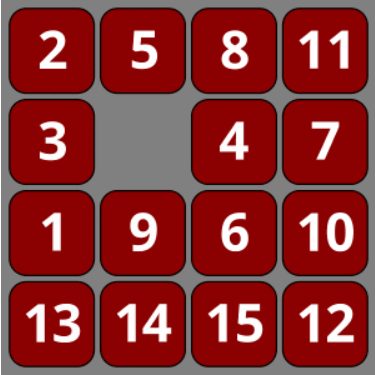
\includegraphics[width=0.3\textwidth]{Pic/1}
      \caption{Searching by IDA*}
    \end{figure}
  \end{block}
\end{frame}


\begin{frame}
  \frametitle{Task}
  \begin{block}{Input-output}
    \begin{itemize}
      \item Input: a 4x4 matrix of initial state.
      \item Output: the path from the initial state to the terminate state.
    \end{itemize}
  \end{block}
  \begin{block}{Submission}
    pack your report \texttt{E02\_YourNumber.pdf} and source code into zip file \texttt{E02\_YourNumber.zip}, then send it to \texttt{ai\_course2021@163.com}.
  \end{block}
\end{frame}

\begin{frame}
  \frametitle{Solution}
  Algorithm procedure
  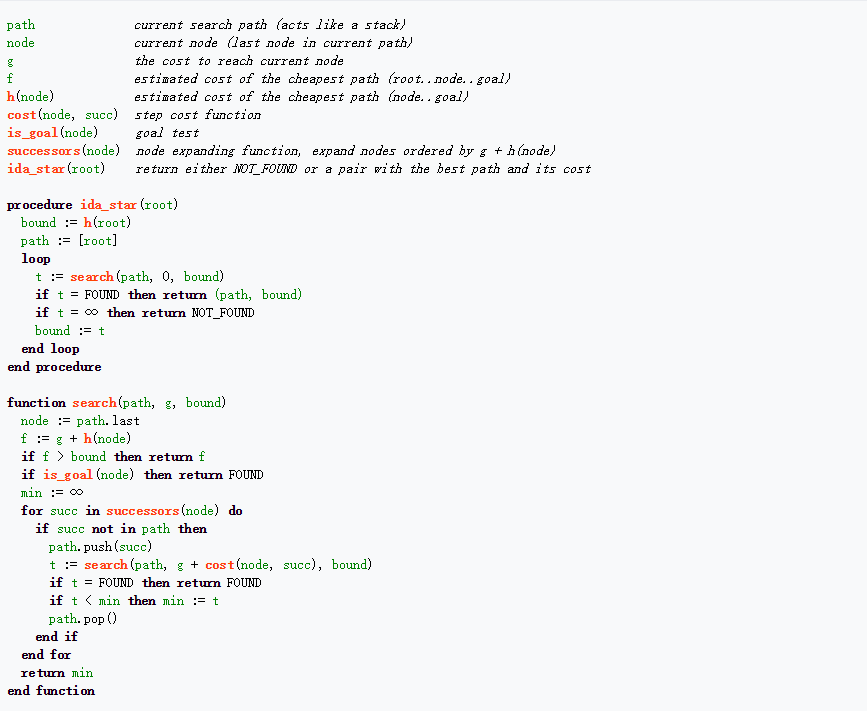
\includegraphics[width=0.8\textwidth]{Pic/code}
\end{frame}

\begin{frame}
  \frametitle{Solution}
  Algorithm illustration
  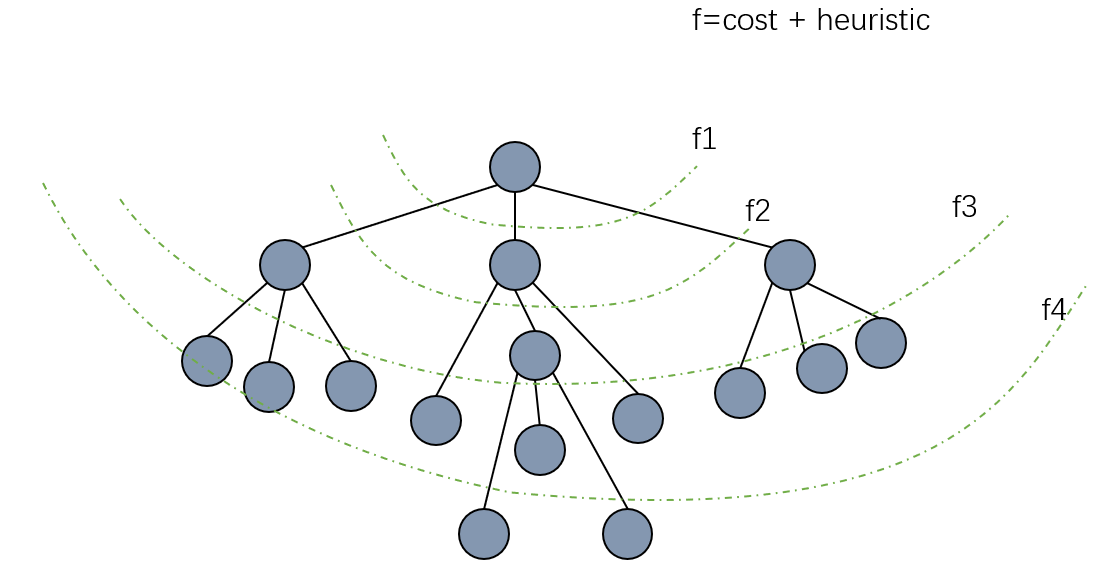
\includegraphics[width=0.8\textwidth]{Pic/ida-star-illustration}
\end{frame}


\begin{frame}
  \frametitle{Solution}
  \begin{columns}
    \begin{column}{.5\linewidth}
      Read input
      
      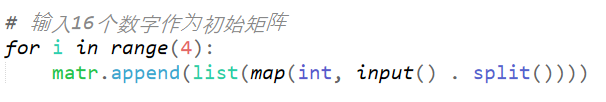
\includegraphics[width=1.1\textwidth]{Pic/read-input}

      Visualize output
      
      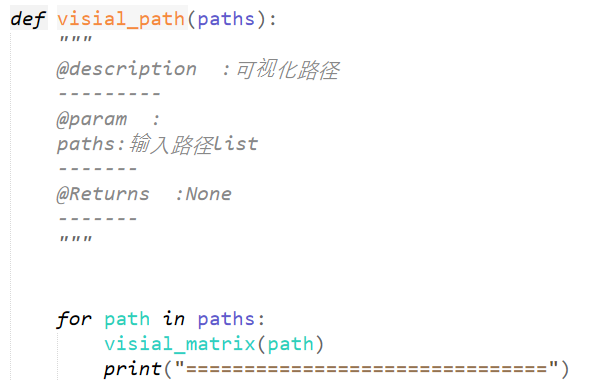
\includegraphics[width=1.0\textwidth]{Pic/visualize-output}
    \end{column}
    \begin{column}{.5\linewidth}
      Get next state
      
      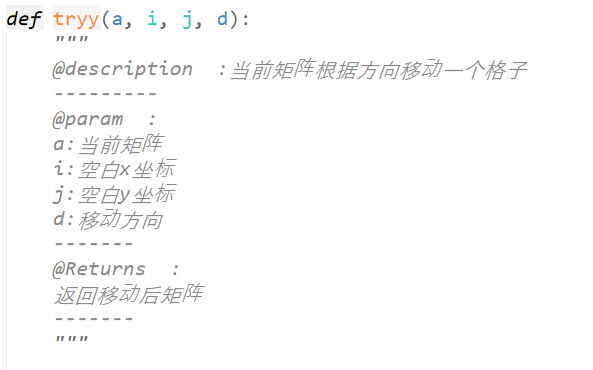
\includegraphics[width=1.1\textwidth]{Pic/get-next-state}
    \end{column}
  \end{columns}

\end{frame}

\begin{frame}
  \frametitle{Solution}
  \begin{columns}
    \begin{column}{.5\linewidth}
      Heuristic 1
      
      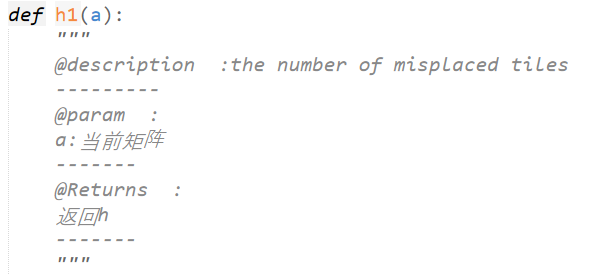
\includegraphics[width=1.0\textwidth]{Pic/h1}

      Heuristic 2
      
      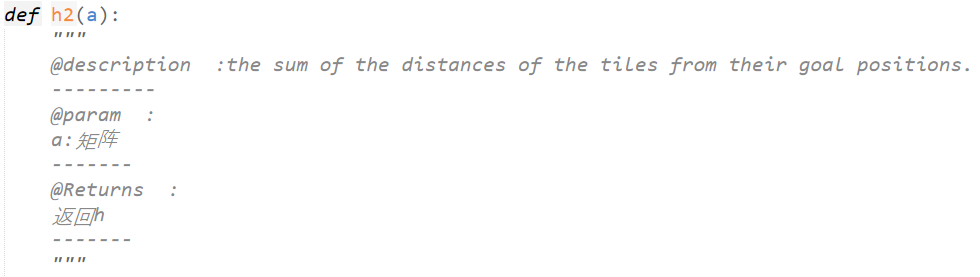
\includegraphics[width=1.8\textwidth]{Pic/h2}
    \end{column}
    \begin{column}{.5\linewidth}
      Search
      
      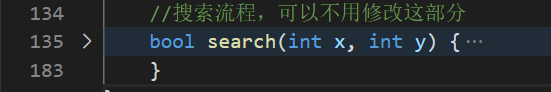
\includegraphics[width=1.1\textwidth]{Pic/search}
    \end{column}
  \end{columns}

\end{frame}
%-----------------------------------------------------------------------------------------

\begin{frame}
  \Huge{\centerline{The End}}
\end{frame}

% ----------------------------------------------------------------------------------------


\end{document}
